\subsection{Results}

\begin{figure*}[ht]
    \centering
    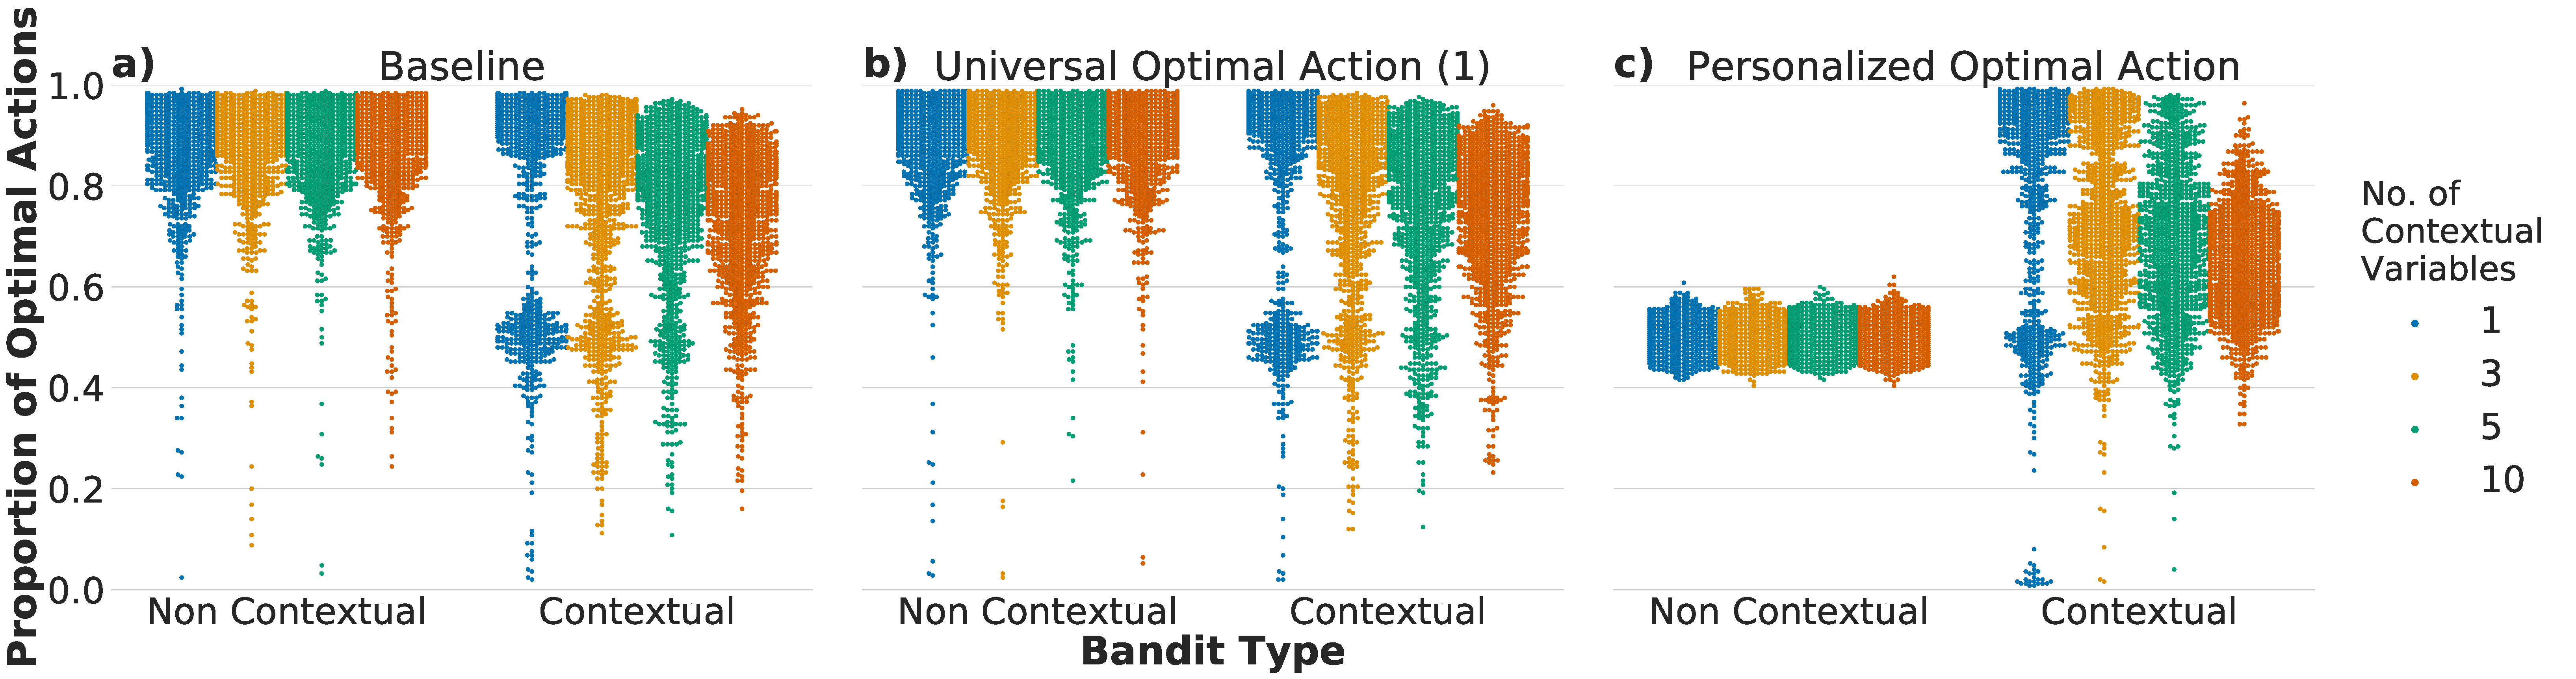
\includegraphics[width=\textwidth]{figs/NumConvars.pdf}
    \caption{Swarm plots for the proportion of optimal actions for the two bandit types. Each point represents results from one trial with 250 students. For the universal optimal action, all scenarios show similar results; hence only scenario (1) is shown. The decreased performance of the contextual bandits in the baseline and universal optimal action scenarios, especially for large number of contextual variables, highlights the potential risks of personalization.}
    \label{fig:NumConVars}
\end{figure*}

\begin{table*}[ht]
\begin{tabular*}{\textwidth}{@{\extracolsep{\fill}}llrlrlr}
\toprule
{} & Superior bandit &  $|b|$ &         95\% CI &  $F(1, 13996)$ &       $p$ &  Cohen's $d$ \\
\midrule
Baseline     &  Non Contextual &  0.098 &  [0.089, 0.108] &         2678.0 &  $< .001$ &        0.871 \\
Universal optimal action (1) &  Non Contextual &  0.088 &  [0.079, 0.097] &         2750.0 &  $< .001$ &        0.880 \\
Universal optimal action (2) &  Non Contextual &  0.078 &  [0.072, 0.085] &         3853.0 &  $< .001$ &        1.042 \\
Universal optimal action (3) &  Non Contextual &  0.101 &   [0.092, 0.11] &         2891.0 &  $< .001$ &        0.904 \\
Universal optimal action (4) &  Non Contextual &  0.074 &  [0.063, 0.085] &         1865.0 &  $< .001$ &        0.725 \\
Personalized optimal action       &      Contextual &  0.295 &  [0.287, 0.302] &        10816.0 &  $< .001$ &        1.677 \\
\bottomrule
\end{tabular*}


\caption{Inferential statistics for proportion of optimal actions for the two bandit types across all outcome-generating models, simulated for 1000 trials of 250 students each. $b$ represents the coefficient of improvement of results for the superior bandit after controlling for the number of contextual variables.}
\label{table:resultsNumConVars}

\end{table*}

\begin{figure}[ht]
    \centering
    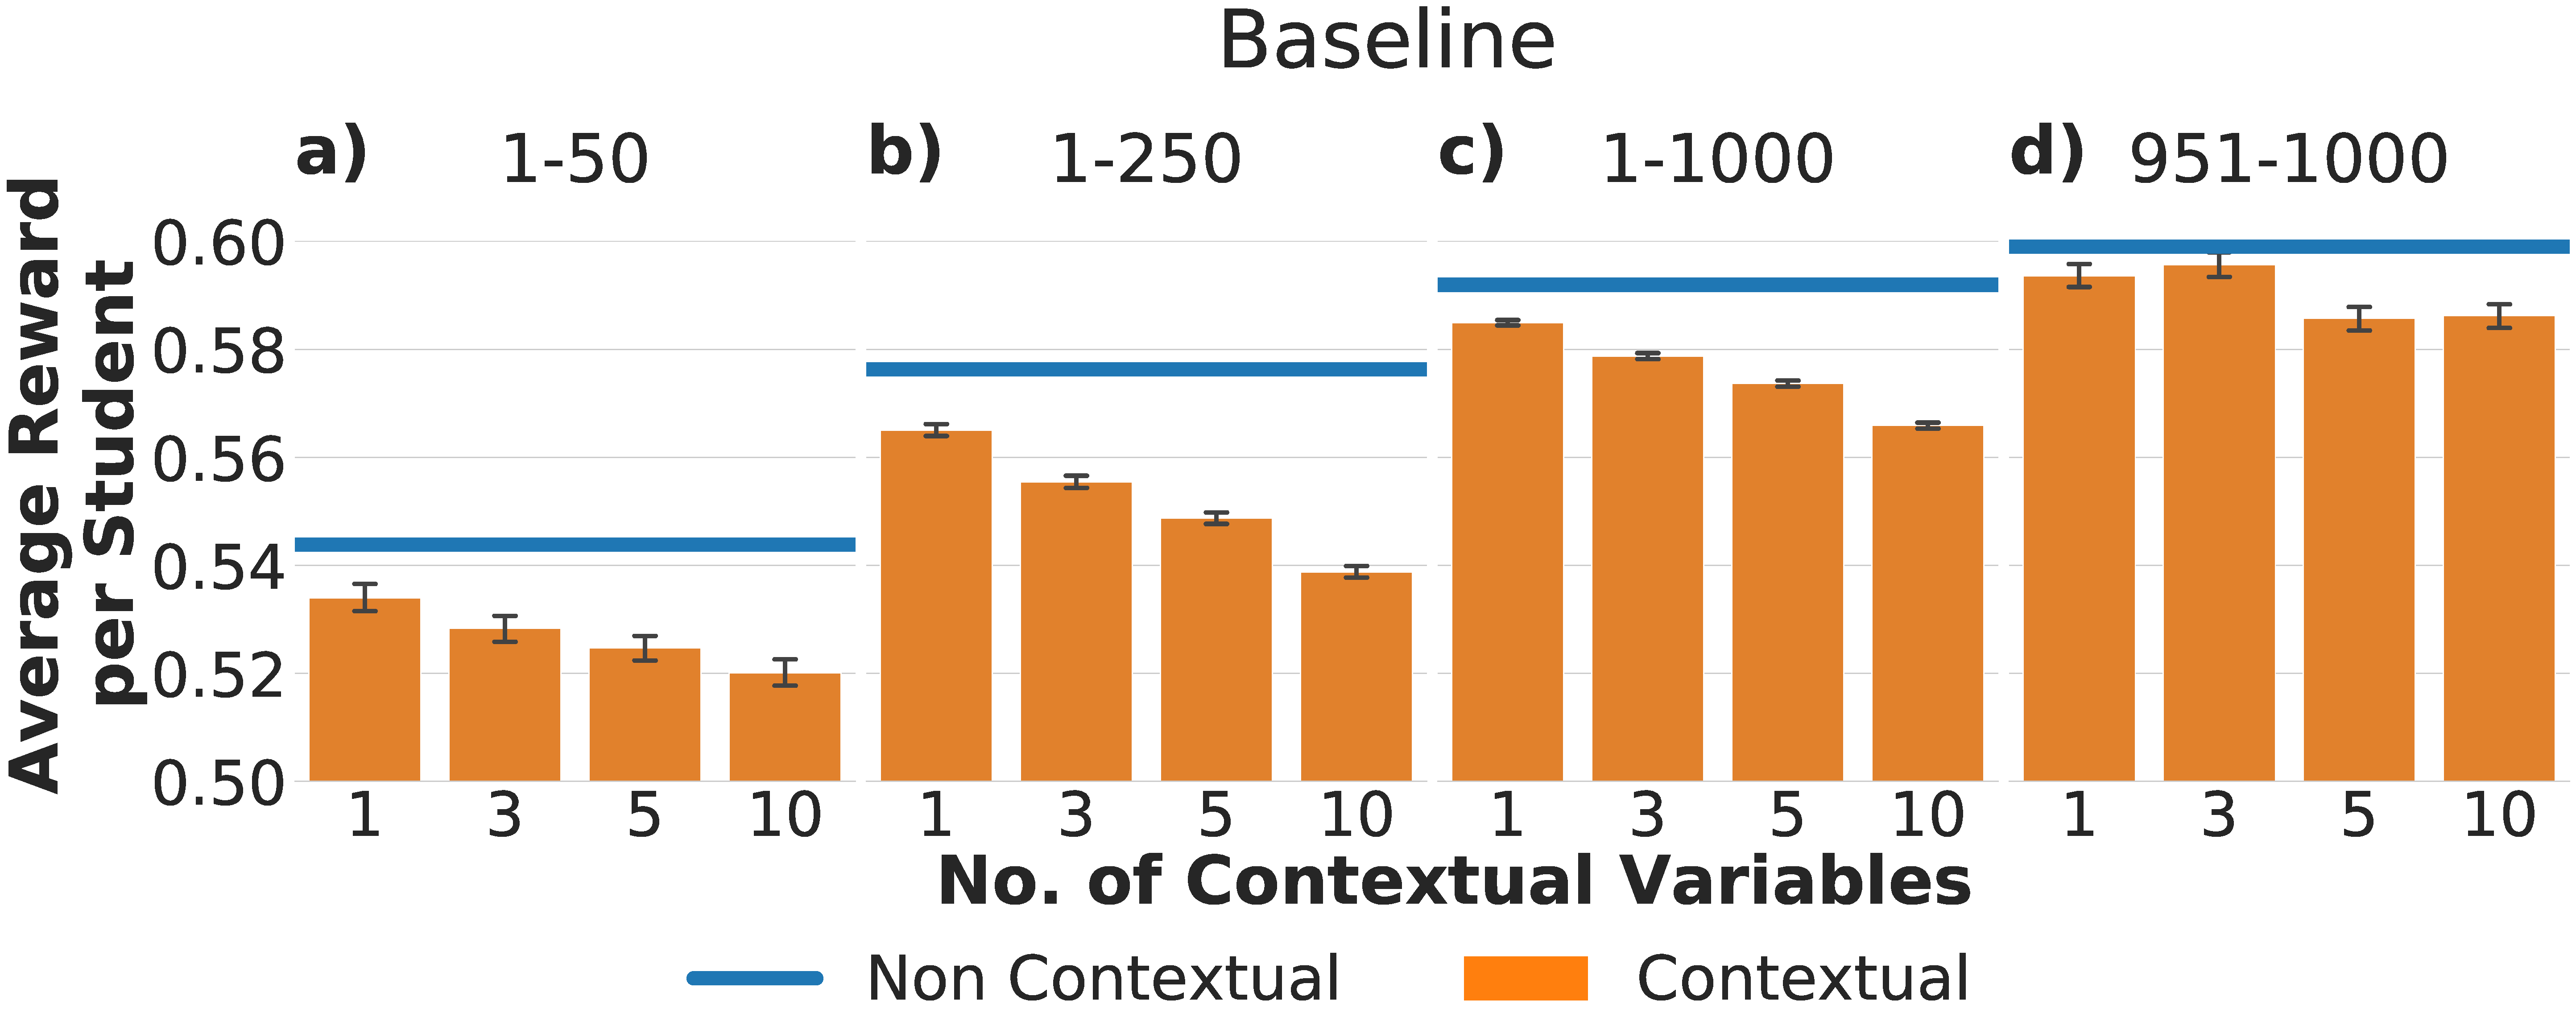
\includegraphics[width=\columnwidth]{figs/NumConVarsRanges.pdf}
    \caption{Average reward per student across 1--10 contextual variables for the two bandit types in the baseline model. In this model, the maximum possible expected reward is $0.6$, and the expected reward for uniform random assignment is $0.5$.
    % The bar graphs for the 4 time horizons are generated by simulating 1000-student classrooms over 1000 trials. 
    Error bars represent 1 standard error.}
    \label{fig:NumConVarsRanges}
\end{figure}

First we focused on analyzing the performance of contextual and non-contextual MAB algorithms for the three outcome-generating models across 1 to 10 student features (i.e., contextual variables).
Using an analysis of covariance (ANCOVA), we compared the two MAB algorithms' performance with respect to the proportion of optimal actions for 250 students across 1000 trials, treating the number of contextual variables as a covariate.
%An analysis of covariance (ANCOVA) were used to examine the difference in performance between the two bandit types, in terms of proportion of optimal actions for 250 students averaged over 1000 trials, while controlling for the number of contextual variables.

% The ANOVA model treats the proportion of optimal actions as the dependent variable, and the type of bandit and the number of contextual variables as a categorical and continuous dependent variables respectively

\textbf{Baseline:} When student features do not influence outcomes, we see that as expected, the non-contextual bandit outperforms the contextual bandit (Table~\ref{table:resultsNumConVars}): average performance per student for the final 50 out of 1000 students using the contextual algorithm is similar to that of the first 250 students using the non-contextual algorithm (Figure~\ref{fig:NumConVarsRanges}). 
As the number of student features increases, the contextual MAB chooses a lower proportion of optimal actions for the first 250 students (Figure~\ref{fig:NumConVars}a), but the effect is relatively small especially when considering the impact on actual reward ($t(13996)=-10.880$, $p<0.001$, $b=-0.006$, 95\% CI = $[-0.007, -0.005]$). At longer horizons, the number of student features has less of an impact on overall average reward (Figure~\ref{fig:NumConVarsRanges}), which we discuss more below.
% As shown in Figure~\ref{fig:NumConVarsRanges}, the impact of more student characteristics decreases as the number of students (horizon) increases: early on, more student characteristics necessitate more exploration, but after the algorithm has interacted with a large number of students (right,  Figure~\ref{fig:NumConVarsRanges}), that increased exploration early has resulted in higher rewards, as the extra exploration is likely to have resulted in more accurate estimates for how actions, student characteristics, and outcomes are related.


\textbf{Universal optimal action:} When outcomes are dependent on student features, the contextual MAB algorithm can learn a more accurate model than the non-contextual algorithm. However, when this more accurate model is not \textit{needed} for optimal action choices, learning the more accurate model does not improve action choices: the non-contextual bandit outperforms the contextual bandits in all four scenarios (Table~\ref{table:resultsNumConVars}; see Figure~\ref{fig:NumConVars}b for scenario 1).  While each scenario might arise due to different educational conditions, they are all very similar in how they appear to the non-contextual bandit algorithm.
The non-contextual bandit sees the two groups of students as identical, leading the overall performance to be the average for each group.
These changes in the average effectiveness of each intervention impact the algorithm's performance but do not necessarily degrade that performance; instead, the impact is dependent on how similar the two interventions are in their expected outcomes and how close those expected outcomes are to $0.5$, where there is the most variance.

\textbf{Personalized optimal action:} When the best policy for individual students depends on their features, the contextual bandit significantly outperforms the non-contextual bandit (Table~\ref{table:resultsNumConVars}). When only one student feature is included, the contextual MAB algorithm chooses the optimal action almost 70\% of the time for the first 50 students; this increases to almost 90\% for the final 50 of the total 250. Including extra student features decreases performance - if ten features are included and only one impacts the policy, the overall proportion of optimal actions falls to about 65\%. Yet, this is still an improvement over the non-contextual algorithm (Figure~\ref{fig:NumConVars}c).
These results suggest that even if a relatively small number of students will interact with the system and one is uncertain about which of a (limited) set of features will impact results, including those features will on average have a positive impact on student outcomes if one is confident that the best version of the system for an individual student varies based on one of those features.



\textbf{Variability across simulations:} Examining variability across simulations provides insight into how likely actual deployments of these algorithms are to reflect their average performance. Across all models, the contextual MAB algorithm exhibited greater variability in performance than the non-contextual MAB algorithm (Figure~\ref{fig:NumConVars}).
% more variability means that in many cases, the results may drift significantly from the averages, based on the variability in student responses. 
% While only the scenario involving a personalized optimal action resulted in better performance for the contextual MAB algorithm, variability of the contextual MAB algorithm's performance was consistently higher than the variability for the non-contextual MAB algorithm's performance. 
Surprisingly, increasing the number of student features leads to lower variance for the contextual MAB algorithm.  With small numbers of student features, there is often a concentration of simulations with lower achieved outcomes, resulting in bimodal distributions (Figure~\ref{fig:NumConVars}).   
The bimodality emerges because the algorithm can adapt more quickly, making it somewhat more vulnerable to underestimating parameter values based on a few samples with unexpected low rewards. Because the parameter estimates influence future action choices, data to correct these underestimates may not be collected quickly enough (as has been documented for non-contextual bandits in, e.g.,~\cite{erraqabi2017trading}). In contrast, increasing the number of student features increases variation near the mean but eliminates the bimodality (Figure~\ref{fig:NumConVars}) since the algorithm performs more exploration to learn the larger number of parameters. This makes it less likely to collect data that lead to erroneous conclusions about the effectiveness of actions. Errors in the parameter values are more likely to be corrected because they are unlikely to lead to the same choices for all student features, hence creating more variability in action choice for students with a specific value of a single feature. Indeed, the simulation results support these interpretations: for the baseline and universal optimal action models in a 1000-student classroom (see Figure~\ref{fig:NumConVarsRanges} for baseline), average reward for the first 250 students is lower but reward for the final 50 students is higher as the number of contextual variables increases.  There is thus a trade-off between expected outcomes and variability: the ability of the contextual MAB algorithm to adapt more quickly when it has fewer features to learn comes at the cost of it being less able to correct for wrong conclusions from small amounts of data.

% ANR: try to add something that explicitly calls out the horizon

% As shown in Table~\ref{table:stdev1Variable} [TODO: change to figure], the outcomes of the simulations using the contextual MAB algorithm are consistently more variable, regardless of the scenario, than the outcomes from the the non-contextual MAB algorithm. 
% \annanotes{would be nice to have the violin-type plots here for looking overall given just 1 variable and then looking at multiple variables just with the contextual and one of the three types of scenarios}

\textbf{Variability in policies across students}:
As noted above, the extra parameters learned by the contextual MAB algorithm lead to the potential for greater variability in action choices within a single simulation. This can systematically affect groups of students when the algorithm attaches spurious relevance to a feature that does not actually impact outcomes. We can see this pattern by examining differences in action probabilities for students who differ only by characteristics that do not impact outcomes: that is, considering all students who have the same value for the first feature, how does the probability of choosing a particular action change based on their different values for the other features?
As the number of contextual variables increases, the average maximum difference in action choice probability between such students also increases from 18--25\% when two student features are included in the model to over 90\% when ten features are included in the model after running through 250 students. This occurs both based on the greater expressivity of the model with more student features and the fact that the model with more student features is likely still learning about the impact of each of these features.
This raises potential concerns about inequity: students who should be treated identically by the system may instead be treated systematically differently, based on features that do not impact how they learn.


% \begin{itemize}
%     \item Want to add something here about in the average simulation with the non-contextual bandit, how different are the policies for students who are actually the same? Probably this gets done at a horizon endpoint, examining range and/or probability of assignment to each condition across students within group 1 as a whole and group 2 as a whole (for no effect, all students since groups don't matter).
% \end{itemize}


% \begin{table*}
% \caption{Proportion of optimal actions chosen by each MAB algorithm, based on the outcome-generating environment. The first three horizons correspond to average behavior across all students, given a fixed number of simulated students, while the final horizon is behavior at the end of the simulation, after the algorithm has learned from the first 950 student interactions. }
% \begin{tabular}{lrrrrr}
%                  &      \multicolumn{4}{}{Horizon}\\

% Quarter                 &      1-50 &      1-250 &              1-1000 &    951-1000 \\
% Bandit and Effect Type  &         &          &                   &                      \\
% ModContextual,None      & 0.69008 & 0.794872 &          0.846208 &              0.86748 \\
% ModContextual,Main (1)  & 0.70622 & 0.815184 &          0.867724 &              0.89082 \\
% ModContextual,Interaction48 &  0.75520 & 0.854288 &          0.893569 &     0.90876 \\
% ModContextual,Interaction57 &  0.69032 & 0.793884 &          0.845840 &     0.87096 \\
% ModContextual,Interaction89 &  0.66630 & 0.784140 &          0.845737 &     0.87476 \\
% ModContextual,Crossover & 0.68280 & 0.818588 &          0.890830 &              0.92334 \\
% NonContextual,None      & 0.73538 & 0.884636 &          0.959528 &              0.99170 \\
% NonContextual,Main (1)  & 0.74018 & 0.892628 &          0.962387 &              0.99172 \\
% NonContextual,Interaction48 &  0.80700 & 0.935956 &          0.979469 &     0.99674 \\
% NonContextual,Interaction57 &  0.73716 & 0.888996 &          0.960632 &     0.99154 \\
% NonContextual,Interaction89 &  0.70072 & 0.849556 &          0.941552 &     0.98550 \\
% NonContextual,Crossover & 0.50132 & 0.501544 &          0.500659 &              0.50000 \\

% \end{tabular}


% % \begin{tabular}{lrrrrr}
% % Quarter                 &      50 &      250 &              1000 &   201-250 &  951-1000 \\
% % Bandit and Effect Type  &         &          &                   &           &                    \\
% % ModContextual,Crossover & 0.68280 & 0.818588 &          0.890830 &   0.88412 &            0.92334 \\
% % ModContextual,Main      & 0.70622 & 0.815184 &          0.867724 &   0.86528 &            0.89082 \\
% % ModContextual,None      & 0.69008 & 0.794872 &          0.846208 &   0.84264 &            0.86748 \\
% % NonContextual,Crossover & 0.50132 & 0.501544 &          0.500659 &   0.50044 &            0.50000 \\
% % NonContextual,Main      & 0.74018 & 0.892628 &          0.962387 &   0.96374 &            0.99172 \\
% % NonContextual,None      & 0.73538 & 0.884636 &          0.959528 &   0.96042 &            0.99170 \\
% % \end{tabular}
% \end{table*}

% \begin{table*}[]
% \caption{Std dev TODO: improve caption, possibly combine with the other}\label{table:stdev1Variable}
% \begin{tabular}{lrrrrr}
% \toprule
% Quarter                 &        50 &      250 &             1000 &     201-250 &           951-1000 \\
% Bandit and Effect Type  &           &          &                   &             &                    \\
% ModContextual,Crossover &  0.212184 & 0.223219 &          0.207602 &    0.234230 &           0.210382 \\
% ModContextual,Main      &  0.216981 & 0.207370 &          0.204598 &    0.221534 &           0.208289 \\
% ModContextual,None      &  0.209366 & 0.218559 &          0.218536 &    0.238622 &           0.225952 \\
% NonContextual,Crossover &  0.072406 & 0.030994 &          0.015282 &    0.070336 &           0.071079 \\
% NonContextual,Main      &  0.199207 & 0.106869 &          0.046308 &    0.082158 &           0.034881 \\
% NonContextual,None      &  0.192135 & 0.104140 &          0.034901 &    0.067599 &           0.017246 \\
% \bottomrule
% \end{tabular}
% \end{table*}

% \annanotes{table we want here: proportion optimal action for contextual vs non-contextual at horizons of 0-50, 200-250, 0-250, 950-1000, 0-1000. Want this for all 5 scenarios. Idea is that gives us a sense of relatively short horizons (course with 50 students), medium horizon (course with 250 students, including difference in experience for initial and final students who interact with the system), and long horizon (course with 1000 students). Then also make this table for reward. For the group dependent reward scenarios, it would be nice to have another table that includes the same horizons but is just looking at the following alg/env: context, non-context, average of non-context with horizons halved and only one of the groups included (basically, removing the noise but retaining the mix of rewards - need to think about this one a little more, since it's sort of the separate contextual case...; maybe also compare to the same horizons but with one set of rewards or the other - that's asically an upper bound on how well we'd expect to do). Currently making that first table, although I think I'm likely missing a couple of the scenarios and will need to add them in. Need to run the simulations for the second non-contextual cases for that second table [this is currently happening].}


% \annanotes{
% To remake graphs in spring 2019 writeup:
% Summary_Statistics_PosterData_Clean_ModANR.ipynb : creates the data frame, including grabbing the appropriate students for each quarter (note that remaking the data frame takes a while)

% Bandit_Stats_Comparison_Graphing.ipynb: does the actual graphing based on the data frame created by the notebook above
% }
% \textbf{One contextual variable}\newline


% \vfill % Delete this to get rid of the column break!